\documentclass[dvipdfmx,11pt]{beamer}
\usepackage{lipsum}
\usetheme{EastLansing}
\usepackage{bxdpx-beamer}
\usepackage{pxjahyper}
\usepackage{minijs}
\usepackage{mathpazo}
\usepackage{amsmath,amssymb}
\usepackage{graphicx}
\usepackage{array}
\usepackage{tikz}
\usepackage{wrapfig}
\usepackage{float}
\usepackage{here}
\usepackage{lscape}
\usepackage{siunitx}
\setbeamertemplate{navigation symbols}{}

\title{Effects of parental leave policies \\ on female career and fertility choices}
\subtitle{Yamaguchi (2019, Quantitative Economics)}
\author{Reio TANJI}
\date{June 19th, 2020}
\institute{Osaka University, Graduate School of Economics}

\begin{document}
\begin{frame}\frametitle{}
\titlepage
\end{frame}

\section{Introduction}
\subsection{Abstract}

\begin{frame}\frametitle{Abstract}
  This paper explores the effect of the parental leave (PL) legislation in Japan.
  \begin{itemize}
    \item Using structual dynamic discrete choice model of female employment and fertility decisions, this paper constructs counterfactual simulations of policy reform of PL legislation.
    \begin{itemize}
      \item The duration of job-protected leave
      \item The replacement rate of cash benefits
    \end{itemize}
    \item 1-year job protection increases maternal employment, while extending the duration of job protection from 1 to 3 years has little effect.
  \end{itemize}
\end{frame}

\begin{frame}\frametitle{Introduction}
  \begin{itemize}
    \item Parental leave, or \textbf{PL}, is mandated in most developed countries, but the generocity of PL legislation varies significantly across countries.
    \item Policy makers are interested in expanding their PL policies to rersolve the conflict between work and family life.
    \item Possible way to predict likely outcomes before a policy reform:
    \begin{itemize}
      \item to learn from the experiences of countries where the most generous PL policies are already mandated: not fully generalized
      \item to conduct a small-scale social experiment: costly and politically infeasible.
    \end{itemize}
    \item To approach to ex ante policy evaluation, this paper constructs a \textbf{structual dynamic discrete choice model} of women's employment and fertility.
  \end{itemize}
\end{frame}

\begin{frame}\frametitle{}
  \begin{figure}
    \centering
    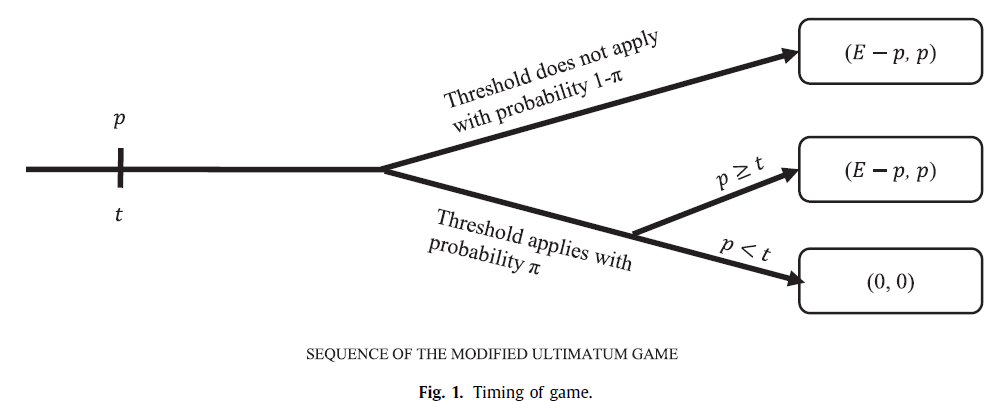
\includegraphics[scale = .54]{0619tanji_fig/F1}
    \label{F1}
  \end{figure}
\end{frame}

\begin{frame}\frametitle{Summary of Results}
  \begin{itemize}
    \item The counterfactual simulations
    \begin{itemize}
      \item 1-year job protection increases maternal employment after childbearing with effects that last for several years, compared with no mandated PL.
      \begin{itemize}
        \item Job protection allows women to suspend working prior to childbirth without losing their jobs: no entry costs to return to work.
      \end{itemize}
      \item Extending the duration of job protection from 1 to 3 years has little effect.
      \begin{itemize}
        \item Nonpecuniary utility of work is very negative when the child is newborn but becomes much smaller as the child grows to age 1 year or older.
      \end{itemize}
      \item Policy effects on fertility seem modest for both 1- and 3-year job protection.
      \item Raising the rate of cash benefits that accrue with job-protected PL has modest effects on maternal work and fertility.
    \end{itemize}
  \end{itemize}
\end{frame}

\subsection{Literature and Contribution}

\begin{frame}\frametitle{Contribution}
  \begin{itemize}
    \item To use a structural estimation approach to evaluate potential PL reforms.
    \begin{itemize}
      \item to learn from the experiences of countries where the most generous PL policies are already mandated: not fully generalized
      \item to conduct a small-scale social experiment: costly and politically infeasible.
    \end{itemize}
    \item Previous approach:
    \begin{itemize}
      \item difference-in-differences (DID) estimator (Ruhm (1998), Baum (2003a), and Baker and Milligan (2008a))
      \item regression discontinuity designs (Lalive and Zweimu\"{u}ller (2009), Sch\"{o}nberg and Ludsteck (2014), and Lalive, Schlosser, Steinhauer, and Zweim\"{u}ller (2014))
    \end{itemize}
    \item The structural model helps one understand how PL policies affect maternal work and speculate about the potential policy effects in a given country.
  \end{itemize}
\end{frame}

\begin{frame}\frametitle{}
  \begin{itemize}
    \item Related papers
    \begin{itemize}
      \item Eckstein and Wolpin (1989), van der Klaauw (1996), Altug and Miller (1998), Francesconi (2002), Sheran (2007), Keane and Wolpin (2007, 2010), Adda, Dustmann, and Stevens (2017), and Gayle andMiller (2012).
    \end{itemize}
  \end{itemize}
  \begin{itemize}
    \item Technical: Combining following three methods:
    \begin{enumerate}
      \item Kasahara and Shimotsu (2011): allows for permanent unobserved heterogeneity.
      \item Arcidiacono and Jones (2003): Expecation-Maximization algorithm
      \item Aecidiacono, Beyer, Bugni, and James (2013): approximation method for the value function.
    \end{enumerate}
  \end{itemize}
\end{frame}

\section{Institutional Background}

\begin{frame}\frametitle{Background}
  History of PL
  \begin{itemize}
    \item PL in Japan was first enforced in 1992.
    \begin{itemize}
      \item Until 2005 it was eligible for only regular workers.
    \end{itemize}
    \item Cash benefits were first introduced in 1995.
    \begin{itemize}
      \item Cash benefits are not financed by employment insurance (same as Austria, Canada, and Germany).
      \item Cash benefits are tied to the job from which PL is taken.

      $\Rightarrow$ PL takers are expected to return to the pre-leave job.
      \begin{itemize}
        \item PL takers must apply through employers to receive cash benefits
        \item Although there is no legal penalty for not returning, about 90\% of PL takers are employed 1 year after childbearing
      \end{itemize}
    \end{itemize}
  \end{itemize}
\end{frame}

\begin{frame}\frametitle{}
  \begin{figure}[h]
    \centering
    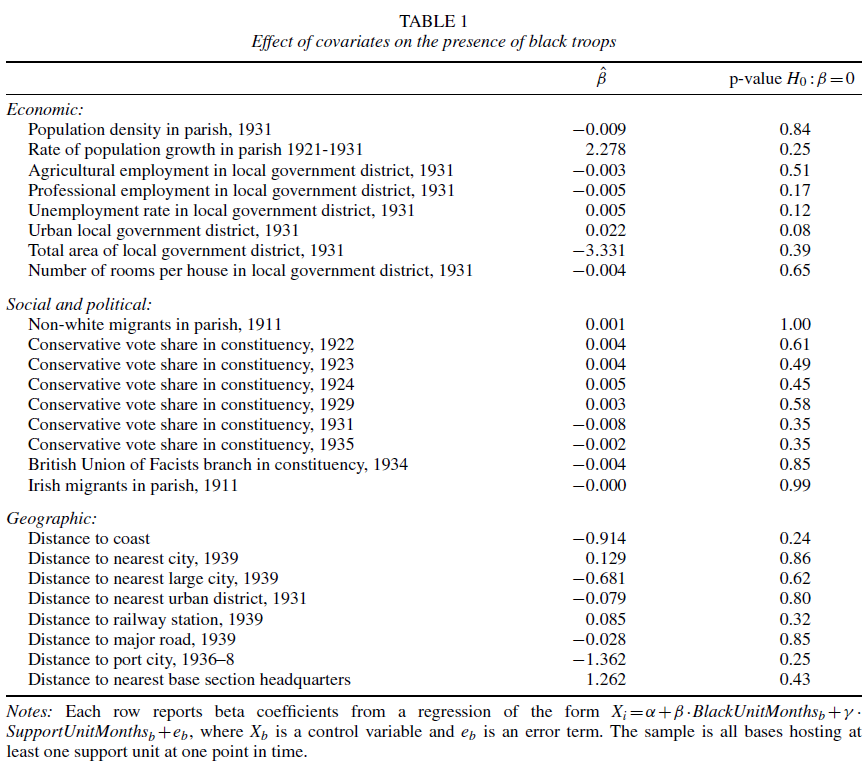
\includegraphics[scale = .6]{0619tanji_fig/T1}
    \label{T1}
  \end{figure}
  \begin{itemize}
    \item Notes
    \begin{itemize}
      \item If a PL taker gives birth during her leave, she can renew the PL and receive cash benefits.
      \item Very few fathers take PL. In 2010, the PL takeup rate among fathers was 1.38\%, and more than half of male PL takers were on leave for only 1 week.
    \end{itemize}
  \end{itemize}
\end{frame}

\section{Data}
\subsection{Overview of the data structure}

\begin{frame}\frametitle{Data}
  Japanese Panel Survey of Consumers (JPSC) by The Institute for Research onHousehold Economics.
  \begin{itemize}
    \item A panel survey of a representative sample of women aged 24-52
    \item started in 1993, with 1,500 women aged 24-34
    \item asks about: every year
    \begin{itemize}
      \item marriage, fertility
      \item their and their spouse's work.
    \end{itemize}
    \item As of 2008, the JPSC had sampled 2,284 women.
    \item Observation period: 1993 - 2011
  \end{itemize}
\end{frame}

\begin{frame}\frametitle{}
  \begin{figure}[h]
    \centering
    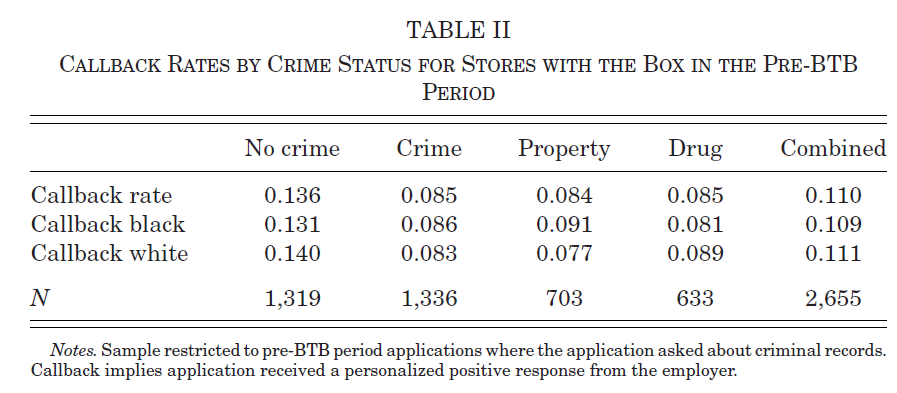
\includegraphics[scale = .5]{0619tanji_fig/T2}
    \label{T2}
  \end{figure}
  \begin{itemize}
    \small
    \item A sample of married women who completed schooling and were not employed.
    \item Observation with missing values except for self-earnings are omitted.
    \item $N = 14,907$ person $\times$ year.
  \end{itemize}
\end{frame}

\subsection{Descriptive analysis}
\begin{frame}\frametitle{}
  \begin{figure}[h]
    \centering
    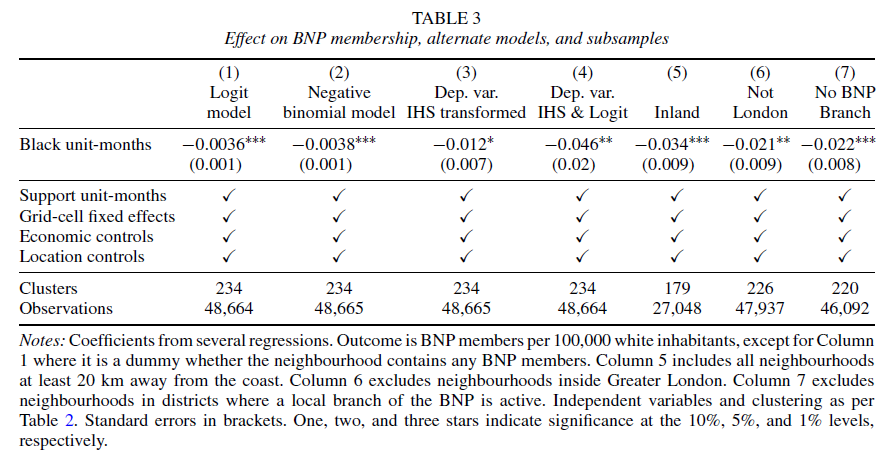
\includegraphics[scale = .5]{0619tanji_fig/T3}
    \label{T2}
  \end{figure}
  Life-cycle profiles
  \begin{itemize}
    \small
    \item Women gradually return to the labor market after childbearing, but largely to nonregular employment.
    \item The percentage of PL takers is small, at 3.7\% at age 30 years, and gradually decreases with age.
    \item Self and husbandsearnings increase over time.
  \end{itemize}
\end{frame}

\begin{frame}\frametitle{}
  Employment transition
  \begin{figure}[h]
    \centering
    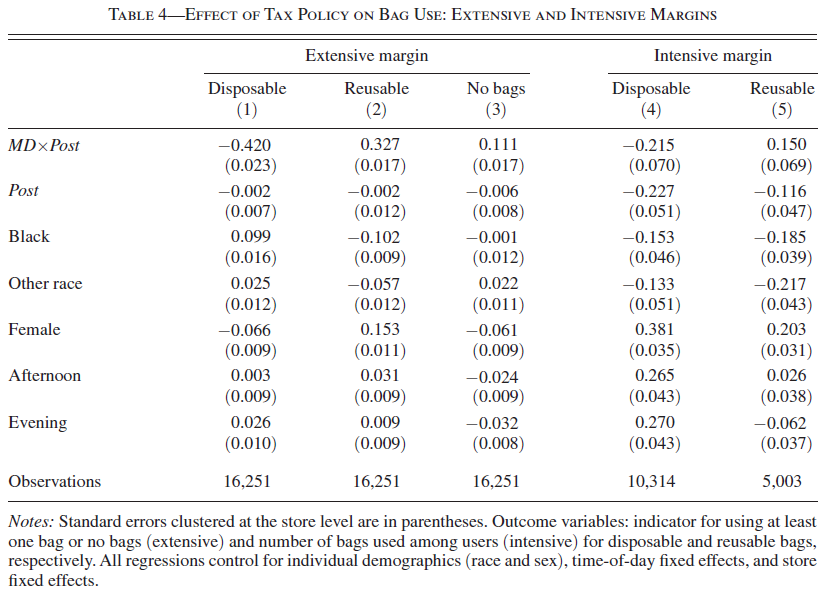
\includegraphics[scale = .6]{0619tanji_fig/T4}
    \label{T2}
  \end{figure}
  \begin{itemize}
    \small
    \item The vast majority of PL takers in $t - 1$ return to work in $t$.
    \item Employment choices are serially correlated except for PL.
    Possible sources:
    \begin{itemize}
      \footnotesize
      \item heterogeneity
      \begin{itemize}
        \item sector-specific human capital
        \item an entry barrier to employment sectors
      \end{itemize}
      \item state dependence
    \end{itemize}
  \end{itemize}
\end{frame}

\begin{frame}\frametitle{}
  PL take-up rate

  \begin{itemize}
    \begin{figure}[h]
      \centering
      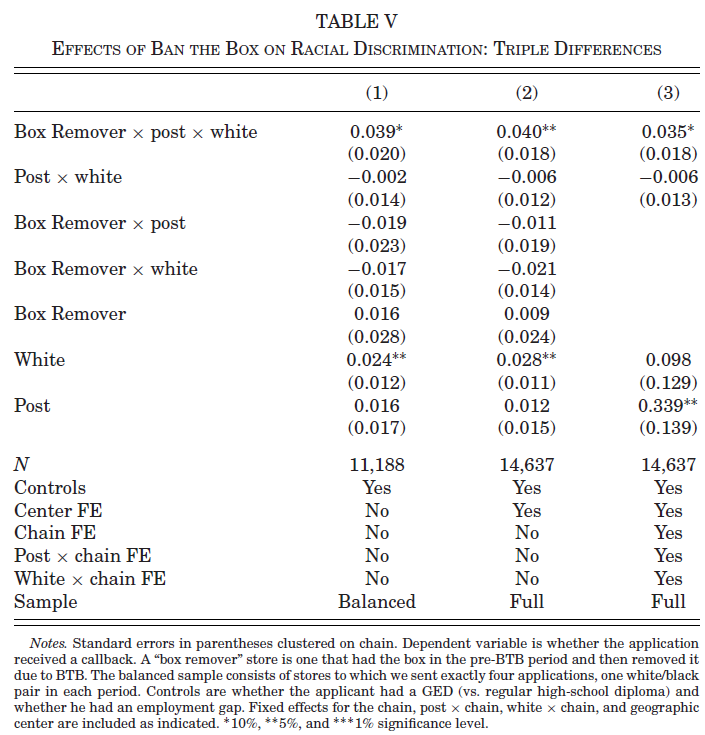
\includegraphics[scale = .6]{0619tanji_fig/T5}
      \label{T2}
    \end{figure}
    \footnotesize
    \item Among women who give birth, only about 30\% hold a job eligible for PL at childbirth.
    \item Although there is no penalty for not returning, about 90\% of leave takers return to employment a year after childbearing
    \begin{itemize}
      \item about 30\% actually end up quitting their jobs without collecting cash benefit
    \end{itemize}
  \end{itemize}
\end{frame}

\end{document}
